% !TeX program = xelatex
% !TeX encoding = UTF-8
\documentclass{MathorCupModeling}
\usepackage{mwe,color,float}
\usepackage[linesnumbered,ruled]{algorithm2e}
\everymath{\displaystyle}

\extrafloats{100}
\bianhao{MC2305806}
\tihao{D}
\timu{\textbf{题目}}
\keyword{关键词两个之间分号隔开}
\begin{document}
	\begin{abstract}
		这里是摘要部分
	\end{abstract}

	\pagestyle{empty}
	\tableofcontents
	\newpage
	\pagestyle{fancy}

	\setcounter{page}{1}
	\section{问题的提出}
	\subsection{问题背景}
	改革开放以来,我国民航业蓬勃发展,越来越多的乘客选择乘坐飞机出行,飞行安全的重要性不言而喻。截至2022年3月21日,即“3.21”空难发生前,我国民航安全飞行达1亿零59万飞行小时,为我国历史最好安全记录。严重的飞行安全事故不仅会使航空公司蒙受经济损失,还威胁着乘客的生命财产安全。为科学管理,降低飞行事故发生的几率,综合现有数据进行监测并预警风险,总结出具有针对性和系统性的方案提升从业人员素质显得尤为重要。在航空安全数据分析中快速存取记录器(Quick Access Recoder,QAR)发挥着重要作用。目前我国民航业主要研究两方面:
	\begin{itemize}
		\item 超限事件的研究,分析及应用;
		\item 非超限数据的统计分析及应用。
	\end{itemize}其中,对于前者的分析着眼于超出阈值的部分,然而超出阈值的部分不完全是人为因素,可能为环境或飞机本身存在一定问题,若基于非人为因素对机组严以要求显然是不合理的。QAR超限可为航空安全管理和飞行训练提供数据支撑,而少量的QAR超限显然不具有说服性,故挖掘QAR全航段数据,基于不同飞行机组,航线,机场及特殊飞行条件下的飞行记录,建立数学模型,并分析之,评估各指标风险系数,针对性开展安全培训,排除安全隐患,改进安全绩效。
	\subsection{问题要求}
	\begin{itemize}
		\item \textbf{问题一}:由于QAR数据并不能保证绝对正确性,故应进行数据预处理减少错误数据干扰。在此基础上对附件1进行可靠性研究,提取关键数据项并分析重要程度。
		\item \textbf{问题二}:飞行过程往往通过一系列飞行操纵如:横滚、俯仰等以保证安全。国内航司主要以超限监控飞行动态,虽然能够快速分辨飞机状态偏差,但无法在较短时间内知道原因。为解决此问题,请依据附件1合理量化描述飞行操纵。
		\item \textbf{问题三}:除人为,环境,飞机本身缺陷外等因素外,仍有一定因素会影响超限的发生。请依据附件2分情况讨论超限并研究其基本特征。
		\item \textbf{问题四}:飞机运行数据研究往往由两大类组成,一类由LOSA获取,另一类则遵从相关学者建议,开展飞行技术评估。请依据附件3,建立数学模型以合理分析评估飞行员飞行技术。
		\item \textbf{问题五}:在QAR实现陆空实时传输的情况下,以航司安全管理人员的身份建立实时自动化预警机制,预防可能的安全事故,并依据附件1给出仿真结果。
	\end{itemize}

	\section{问题的分析}
	\subsection{问题的整体分析}
	该问题是一个关于航空安全风险及飞行技术的数据分析、建立预警模型的问题。
	
	\textbf{从分析目的看},

	\textbf{从数据来源、特征看},
	
	\textbf{从模型的选择看},

	\textbf{从编程软件的选择看},本题为大数据分析类,需要进行大量的数据预处理、数据分析、数据可视化,并依据各设问建立预警自动化只能预警机制,因此我们选择Python Jupyter对问题进行求解,其交互式的编程范式及轻量化,方便且高效。
	
	\subsection{问题一的分析}
	问题一的核心目的有以下几点:{\heiti 其一},\textbf{对真实的QAR数据进行预处理,去伪存真};{\heiti 其二},\textbf{分析研究附件一数据质量的可靠性};{\heiti 其三},\textbf{提取一项飞行安全的关键性因素,并定性及定量分析}。对于已给的数据集,数据在真实性、完整度、指标标准等方面存在一定缺陷,这导致我们在原始数据上不可直接进行分析,因此需要对其进行相应的预处理。此外附件1为8次航班的由起飞到降落的全过程的QAR数据,数据体量大,因此我们需要由特殊到一般,建立普适性模型,高效分析多张数据表格;同时我们还发现,数据维度较高,为得到关键性因此,考虑累计方差解释、层次聚类分析及熵权法,确定重要度较高指标,并对筛选出的指标进行合理性分析。
	\subsection{问题二的分析}
	\subsection{问题三的分析}
	\subsection{问题四的分析}
	问题四的核心目的在于\textbf{基于飞行参数对飞行员的技术进行评估}。但是附件3与附件1同样在数据完整度、指标标准等方面存在一定缺陷,因此我们也需要对其进行一定的预处理;同时,我们还发现附件3维度更高,飞行参数较多,对于模型的效率有一定影响,因此我们沿用问题一的想法,以累计方差解释确定重要因素较高的指标的个数,再以随机森林及极端梯度提升算法综合分析出与飞行员飞行技术重要程度较高的因素。但我们还发现,附件3中,飞行员资质为“C”类的占比仅为整体的$0.844\,\%$,因此我们综合多方面考虑,选择将该两项数据单独分析,剩余数据视为多分类预测。最后以筛选出的重要指标为自变量,飞行员的“不同资质”,即不同技术级(除“C”类)别为因变量,建立XGboost多分类预测模型,从而建立出基于飞行参数的飞行技术评估方法。同时,为探讨模型效果,我们绘制出模型的{\heiti 分类混淆矩阵热力图}、{\heiti 分类报告}、{\heiti ROC/AUC	曲线}等对预测结果进行合理性分析。
	\subsection{问题五的分析}

	\section{模型的假设}
	\begin{itemize}
		\item \textbf{假设一}:
		\item \textbf{假设二}:
		\item \textbf{假设三}:
		\item \textbf{假设四}:
	\end{itemize}
	\section{符号说明}
	\begin{center}
		\begin{tabularx}{0.7\textwidth}{c@{\hspace{1pc}}|@{\hspace{2pc}}X}
			\Xhline{0.08em}
			符号 & \multicolumn{1}{c}{符号说明}\\
			\Xhline{0.05em}
			$\mu$ & 样本平均数 \\
			$\alpha$ & 系数 \\
			$\beta$ & \\
			$\omega$ & \\
			$\sigma$ & 标准差 \\
			\Xhline{0.08em}
		\end{tabularx}
	\end{center}

	\section{模型的建立与求解}
	\subsection{问题一模型的建立与求解}





	这里是图片的演示,见\textcolor{blue}{\cref{fig:picturename1}}。
	\begin{figure}[H]
		\centerline{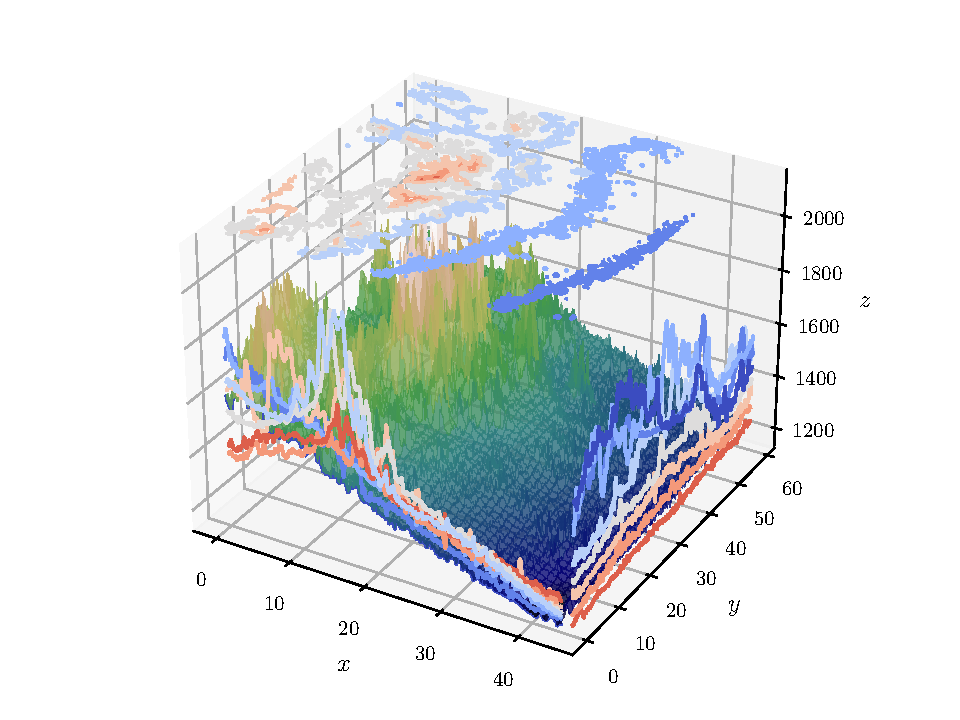
\includegraphics[scale=0.8]{三维网格图.pdf}}
		\caption{这里是图片的标题}\label{fig:picturename1}
	\end{figure}
	这里是第二张图片的延时,见\textcolor{blue}{\cref{fig:picturename2}}。
	\begin{figure}[H]
		\centerline{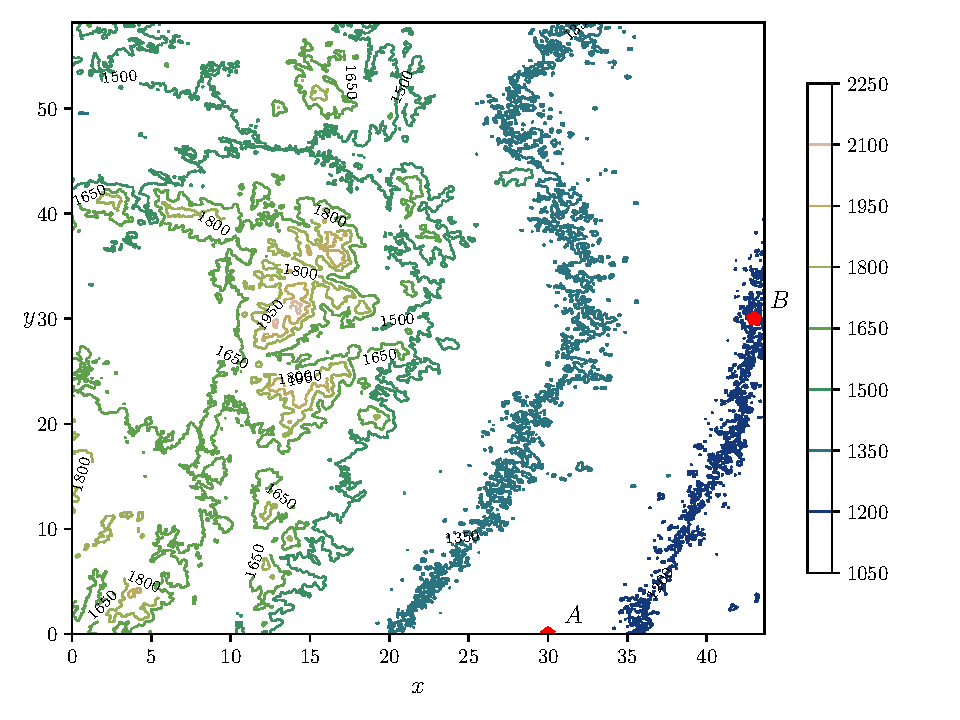
\includegraphics[scale=0.8]{等高线图.pdf}}
		\caption{这里是图片的标题}\label{fig:picturename2}
	\end{figure}
	假如这段话是引用了话,要有注释喔!\textcolor{blue}{\cite{p1}}
	这里我们还可以做个脚注。\textcolor{blue}{\footnote{脚注的内容}}

	这里我们做一个表格,三线表喔!见\textcolor{blue}{\cref{tab:tablename1}}。
	\begin{table}[htbp]
	\centering
	\caption{标题在这里!~}
	\setlength{\aboverulesep}{0pt}
	\setlength{\belowrulesep}{0pt}
	\scalebox{0.88}{
	  \begin{tabular}{ccc}
	  \toprule
	  A     & B     & C \\
	  \midrule
	  1     & 12    & hello \\
	  2     & E     & 汉字 \\
	  3     & apple & pear \\
	  \bottomrule
	  \end{tabular}}
	\label{tab:tablename1}
  	\end{table}
	结果见\textcolor{blue}{\cref{tab:firsttable}}。
	\begin{table}[H]
	\centering
	\caption{表格名称}
	  \begin{tabular}{ccc}
	  \toprule
	  A     & B     & C \\
	  \midrule
	  1     & 2     & 3 \\
	  一     & 二     & 三 \\
	  1     & 2.98  & 3.97 \\
	  \bottomrule
	  \end{tabular}
	\label{tab:firsttable}
 	\end{table}
  % Table generated by Excel2LaTeX from sheet 'Sheet1'
\begin{table}[htbp]
	\centering
	\caption{Add caption}
	\setlength{\aboverulesep}{0pt}
	\setlength{\belowrulesep}{0pt}
	\scalebox{0.5}{
	  \begin{tabular}{c|cc}
	  \toprule
	  A     & B     & C \\
	  \midrule
	  1     & 2     & 3 \\
	  一     & 二     & 三 \\
	  1     & 2.98  & 3.97 \\
	  \bottomrule
	  \end{tabular}}
	\label{tab:addlabel}
  \end{table}
  
这个公式$\frac{x^2}{5}+\frac{y^2}{4}=1$是行内公式
下面的公式为行间公式:
$$
E=\int \frac{\mathrm{d}q}{4\pi \varepsilon_0 r^2}
$$
$$
\sum_{i = 1}^\infty  {\frac{5}{i}}
$$
行内求和$\sum\limits_{i = 1}^\infty  {\frac{5}{i}}$
第二种行间公式如下\textcolor{blue}{\cref{eqone}}
\begin{equation}\label{eqone}
E=\int \frac{\mathrm{d}q}{4\pi \varepsilon_0 r^2}
\end{equation}
	\section{模型的评价与推广}
	\begin{figure}[H]
		\centering{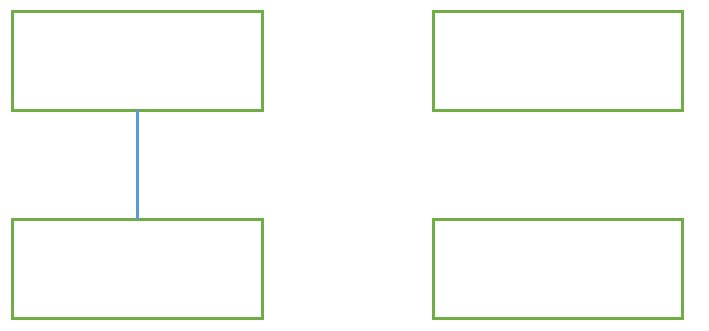
\includegraphics[scale=0.8]{文字文稿1.pdf}}
		\caption{这里是图片的标题}\label{fig:picturename3}
	\end{figure}
	\subsection{模型的评价}
	\begin{itemize}
		\item \textbf{模型的优点}:
			\begin{enumerate}
				\item ……
				\item ……
			\end{enumerate}
		\item \textbf{模型的缺点}:
			\begin{enumerate}
				\item ……
				\item ……
				\item ……
			\end{enumerate}
		\item \textbf{模型的改进}:
			\begin{enumerate}
				\item ……
				\item ……
				\item ……
			\end{enumerate}
	\end{itemize}
	\subsection{模型的推广}

	\newpage
	\phantomsection
	\addcontentsline{toc}{section}{\textbf{参考文献}}
	\begin{thebibliography}{99}
	\bibitem{p1}张学工.关于统计学习理论与支持向量机[J].自动化学报,2000(01):36-46.DOI:10.16383/j.aas.2000.01.005.
	
	\end{thebibliography}

	\newpage

	\phantomsection
	\addcontentsline{toc}{section}{\textbf{附\hspace{2pc}录}}

	% \appendix
	% \ctexset{section={format={\zihao{-4}\heiti\raggedright}}}
	\begin{center}
		\heiti\zihao{4} 附\hspace{2pc}录
	\end{center}

% \phantomsection
% \addcontentsline{toc}{subsection}{[A]图示}
	% \section*{[A]图示}
	\noindent{\heiti [A]图示}

\newpage
% \phantomsection
% \addcontentsline{toc}{subsection}{[B]支撑文件列表}
	% \section*{[B]支撑文件列表}
	\noindent{\heiti [B]支撑文件列表}
	~\\

	支撑文件列表如下(列表中不包含原始数据集):

\newpage
% \phantomsection
% \addcontentsline{toc}{subsection}{[C]使用的软件、环境}
	% \section*{[C]使用的软件、环境}
	\noindent{\heiti [C]使用的软件、环境}
	~\\

	为解决该问题,我们所使用的主要软件有:
	
	Python环境下所用使用到的库及其版本如下:

\newpage
% \phantomsection
% \addcontentsline{toc}{subsection}{[D]问题解决源程序}
	% \section*{[D]问题解决源程序}
\noindent{\heiti [D]问题解决源程序}

% \phantomsection
% \addcontentsline{toc}{subsubsection}{D.1}
\textbf{D.1 }
\begin{python}
import numpy as np
\end{python}
\newpage
% \phantomsection
% \addcontentsline{toc}{subsubsection}{D.2}
\textbf{D.2 }

\newpage
% \phantomsection
% \addcontentsline{toc}{subsubsection}{D.3}
\textbf{D.3 }

\newpage
% \phantomsection
% \addcontentsline{toc}{subsubsection}{D.4}
\textbf{D.4 }

\end{document}